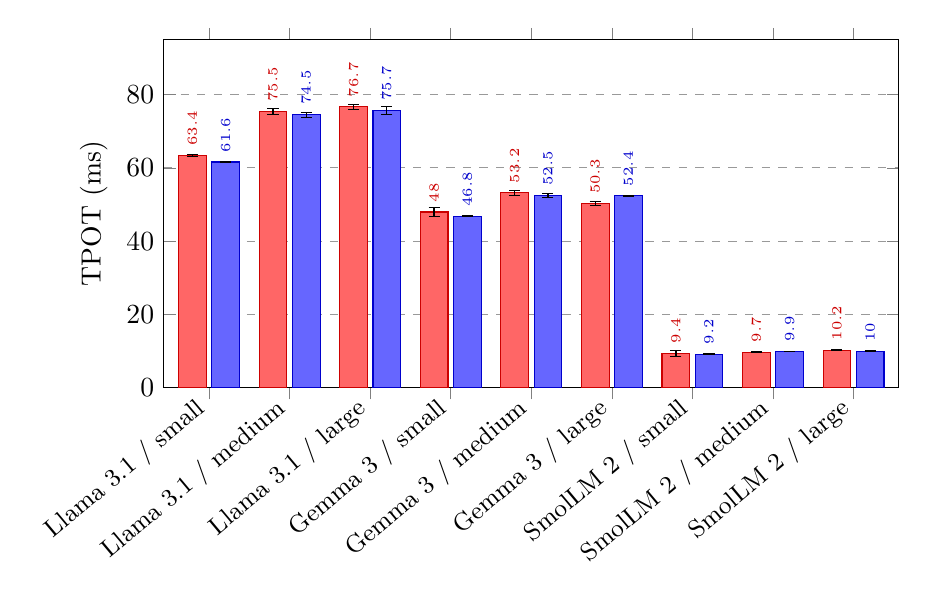
\begin{tikzpicture}
    \begin{axis}[
        % Plot type
        ybar,
        % Plot dimensions
        width            = 0.9\textwidth,
        height           = 6cm,
        enlarge x limits = 0.07,
        % Labels
        ylabel            = {TPOT (ms)},
        symbolic x coords = {
            {Llama 3.1 / small},
            {Llama 3.1 / medium},
            {Llama 3.1 / large},
            {Gemma 3 / small},
            {Gemma 3 / medium},
            {Gemma 3 / large},
            {SmolLM 2 / small},
            {SmolLM 2 / medium},
            {SmolLM 2 / large}
        },
        x tick label style = {rotate = 40, anchor = east, font = \small},
        % Axes
        ymin = 0,
        ymax = 95,
        % Labels
        nodes near coords,
        nodes near coords style={
            font   = \tiny,
            rotate = 90,
            anchor = west,
            /pgf/number format/fixed,
            /pgf/number format/precision = 1
        },
        % Grid
        ymajorgrids = true,
        grid style  = {dashed, gray!80}
    ]

        % --no-mmap data
        \addplot+[
            % Bar and label color
            fill                                = red!60,
            draw                                = red!80!black,
            every node near coord/.append style = {color = red!80!black},
            % Error bars
            error bars/.cd,
            y dir = both,
            y explicit,
            error bar style = {black, line width = 0.5pt},
        ] coordinates {
            ({Llama 3.1 / small},   63.40) +- (0, 0.21)
            ({Llama 3.1 / medium},  75.47) +- (0, 0.78)
            ({Llama 3.1 / large},   76.69) +- (0, 0.64)
            ({Gemma 3 / small},     47.97) +- (0, 1.12)
            ({Gemma 3 / medium},    53.19) +- (0, 0.62)
            ({Gemma 3 / large},     50.25) +- (0, 0.48)
            ({SmolLM 2 / small},     9.43) +- (0, 0.82)
            ({SmolLM 2 / medium},    9.71) +- (0, 0.14)
            ({SmolLM 2 / large},    10.24) +- (0, 0.09)
        };

        % --mmap data
        \addplot+[
            % Bar and label color
            fill                                = blue!60,
            draw                                = blue!80!black,
            every node near coord/.append style = {color = blue!80!black},
            % Error bars
            error bars/.cd,
            y dir = both,
            y explicit,
            error bar style = {black, line width=0.5pt},
        ] coordinates {
            ({Llama 3.1 / small},   61.62) +- (0, 0.25)
            ({Llama 3.1 / medium},  74.54) +- (0, 0.68)
            ({Llama 3.1 / large},   75.68) +- (0, 1.13)
            ({Gemma 3 / small},     46.81) +- (0, 0.07)
            ({Gemma 3 / medium},    52.46) +- (0, 0.59)
            ({Gemma 3 / large},     52.39) +- (0, 0.20)
            ({SmolLM 2 / small},     9.17) +- (0, 0.01)
            ({SmolLM 2 / medium},    9.88) +- (0, 0.09)
            ({SmolLM 2 / large},     9.95) +- (0, 0.10)
        };
    \end{axis}
\end{tikzpicture}
